\subsubsection{Let's forget about MSVC}

In Windows, the \ac{SEH} is intended for exceptions handling, nevertheless, it is language-agnostic,
not related to \Cpp or \ac{OOP} in any way.

Here we are going to take a look at \ac{SEH} in its isolated (from C++ and MSVC extensions) form.

\myindex{Windows!TIB}
\myindex{Windows!Win32!RaiseException()}

Each running process has a chain of \ac{SEH} handlers, \ac{TIB} has the address of the last handler.

When an exception occurs (division by zero, incorrect address access, user exception triggered by
calling the \TT{RaiseException()} function), the \ac{OS} finds the last handler in the \ac{TIB} and calls it,
passing all information about the \ac{CPU} state (register values, etc.) at the moment of the exception.

The exception handler considering the exception, was it made for it?
If so, it handles the exception.

If not, it signals to the \ac{OS} that it
cannot handle it and the \ac{OS} calls the next handler in the chain,
until a handler which is able to handle the exception is be found.

At the very end of the chain there a standard handler that shows the well-known dialog box, informing the user about a
process crash, some technical information about the \ac{CPU} state at the time of the crash,
and offering to collect all information and send it to developers in Microsoft. 

\begin{figure}[H]
\centering
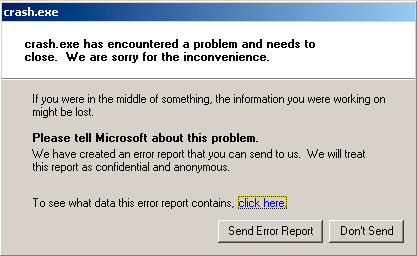
\includegraphics[width=0.6\textwidth]{OS/SEH/1/crash_xp1.png}
\caption{Windows XP}
\end{figure}

\begin{figure}[H]
\centering
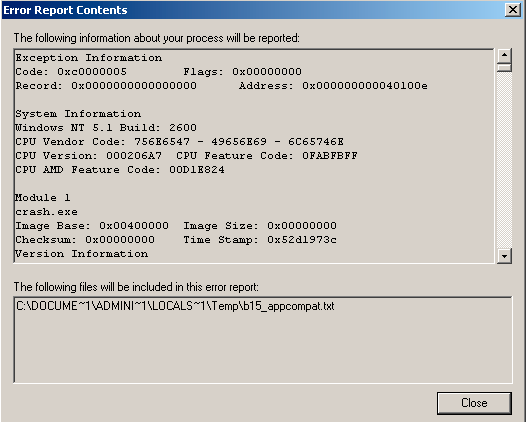
\includegraphics[width=0.6\textwidth]{OS/SEH/1/crash_xp2.png}
\caption{Windows XP}
\end{figure}

\begin{figure}[H]
\centering
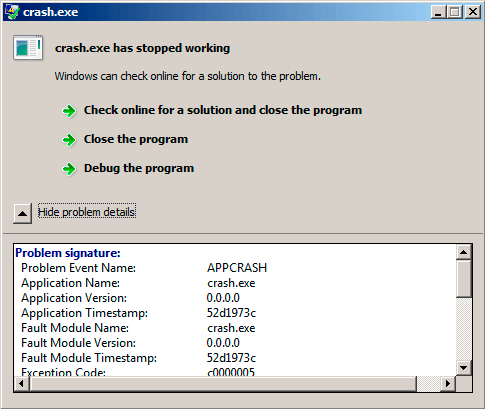
\includegraphics[width=0.6\textwidth]{OS/SEH/1/crash_win7.png}
\caption{Windows 7}
\end{figure}

\begin{figure}[H]
\centering
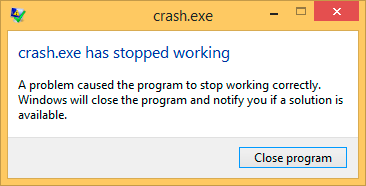
\includegraphics[width=0.6\textwidth]{OS/SEH/1/crash_win81.png}
\caption{Windows 8.1}
\end{figure}

Earlier, this handler was called Dr. Watson
\footnote{\href{http://go.yurichev.com/17046}{wikipedia}}.

By the way, some developers make their own handler that sends information about the program crash to themselves.
\myindex{Windows!Win32!SetUnhandledExceptionFilter()}
It is registered with the help of \TT{SetUnhandledExceptionFilter()} 
and to be called if the \ac{OS} does not have any other way to handle the exception.
\myindex{\oracle}
An example is \oracle---it saves huge dumps reporting all possible information about the \ac{CPU} and memory state.

Let's write our own primitive exception handler.
This example is based on the example from \PietrekSEH.
It must be compiled with the SAFESEH option: \TT{cl seh1.cpp /link /safeseh:no}.
More about SAFESEH here: \href{http://go.yurichev.com/17252}{MSDN}.

\lstinputlisting{OS/SEH/1/1.cpp}

The FS: segment register is pointing to the \ac{TIB} in win32.

The very first element in the \ac{TIB} is a pointer to the last handler in the chain.
We save it in the stack and store the address of our handler there.
The structure is named \TT{\_EXCEPTION\_REGISTRATION}, it is a simple singly-linked list and its elements are stored right in the stack.

\begin{lstlisting}[caption=MSVC/VC/crt/src/exsup.inc]
\_EXCEPTION\_REGISTRATION struc
     prev    dd      ?
     handler dd      ?
\_EXCEPTION\_REGISTRATION ends
\end{lstlisting}

So each \q{handler} field points to a handler and an each \q{prev} field points to the previous record in the stack.
The last record has \TT{0xFFFFFFFF} (-1) in the \q{prev} field.

\begin{center}
\ifdefined\ebook
\begin{tikzpicture}[thick,scale=0.50, every node/.style={scale=0.50}]
\else
\begin{tikzpicture}[thick,scale=0.85, every node/.style={scale=0.85}]
\fi
	\tikzstyle{every path}=[thick]
	\tikzstyle{undefined}=[draw,rectangle,minimum height=1cm, minimum width=3.5cm, text width=3.5cm]
	\tikzstyle{node}=[draw,rectangle,minimum height=1cm, minimum width=3.5cm, text width=3.5cm, fill=gray!20]
	
	\node[node] (fs) [minimum width=1.5cm, text width=1.5cm] {FS:0};

	\node[node] (tib1) [right=1.5cm of fs] {+0: \_\_except\_list};
	\node[undefined] (tib2) [below of=tib1] {+4: \dots};
	\node[undefined] (tib3) [below of=tib2] {+8: \dots};
	\node (tib_text) [above of=tib1] {TIB};
	
	\draw [->] (fs.east) -- (tib1.west);

	\node[undefined] (u1) [text centered, right=2.5cm of tib1] {\dots};
	\node [node] (n1prev) [below of=u1] {Prev=0xFFFFFFFF};
	\node [node] (n1handler) [below of=n1prev] {Handle};
	\node [node] (n1handler_text) [right=1cm of n1handler] {\HandlerFunction};
	\draw [->] (n1handler.east) -- (n1handler_text.west);
	\node[undefined] (u2) [text centered, below of=n1handler] {\dots};
	\node [node] (n2prev) [below of=u2] {Prev};
	\node [node] (n2handler) [below of=n2prev] {Handle};
	\node [node] (n2handler_text) [right=1cm of n2handler] {\HandlerFunction};
	\draw [->] (n2handler.east) -- (n2handler_text.west);
	\node[undefined] (u3) [text centered, below of=n2handler] {\dots};
	\node [node] (n3prev) [below of=u3] {Prev};

	\node [node] (n3handler) [below of=n3prev] {Handle};
	\node [node] (n3handler_text) [right=1cm of n3handler] {\HandlerFunction};
	\draw [->] (n3handler.east) -- (n3handler_text.west);
	\node[undefined] (u4) [text centered, below of=n3handler] {\dots};
	\node (stack_text) [above of=u1] {\IFRU{Стек}{Stack}};
	
	\node (n2block_pt1) [inner sep=0pt, above left=0cm and 0cm of n2prev] {};
	\node (n2block_pt2) [inner sep=0pt, above left=0cm and 0.5cm of n2prev] {};
	\draw [->] (n3prev.west) .. controls +(left:0.5cm) and (n2block_pt2) .. (n2block_pt1);

	\node (n1block_pt1) [inner sep=0pt, above left=0cm and 0cm of n1prev] {};
	\node (n1block_pt2) [inner sep=0pt, above left=0cm and 0.8cm of n1prev] {};
	\draw [->] (n2prev.west) .. controls +(left:0.8cm) and (n1block_pt2) .. (n1block_pt1);
	
	\node (n3block_pt1) [inner sep=0pt, above left=0cm and 0cm of n3prev] {};
	\node (n3block_pt2) [inner sep=0pt, above left=0cm and 1.25cm of n3prev] {};
	\draw [->] (tib1.east) .. controls +(right:1.25cm) and (n3block_pt2) .. (n3block_pt1);


\end{tikzpicture}
\end{center}


After our handler is installed, we call \TT{RaiseException()}
\footnote{\href{http://go.yurichev.com/17253}{MSDN}}.
This is an user exception. 
The handler checks the code.
If the code is \TT{0xE1223344}, it returning \TT{ExceptionContinueExecution},
which means that handler corrected the CPU state (it is usually a correction of the EIP/ESP registers) and the \ac{OS} can resume the execution of the.
If you alter slightly the code so the handler returns \TT{ExceptionContinueSearch},

then the \ac{OS} will call the other handlers, and it's unlikely that one who can handle it will be found, since
no one will have any information about it (rather about its code).
You will see the standard Windows dialog about a process crash.

What is the difference between a system exceptions and a user one? Here are the system ones:

\small
\begin{center}
\begin{tabular}{ | l | l | l | }
\hline
\HeaderColor as defined in WinBase.h & 
\HeaderColor as defined in ntstatus.h & 
\HeaderColor value \\
\hline
EXCEPTION\_ACCESS\_VIOLATION          & STATUS\_ACCESS\_VIOLATION           & 0xC0000005 \\
\hline
EXCEPTION\_DATATYPE\_MISALIGNMENT     & STATUS\_DATATYPE\_MISALIGNMENT      & 0x80000002 \\
\hline
EXCEPTION\_BREAKPOINT                & STATUS\_BREAKPOINT                 & 0x80000003 \\
\hline
EXCEPTION\_SINGLE\_STEP               & STATUS\_SINGLE\_STEP                & 0x80000004 \\
\hline
EXCEPTION\_ARRAY\_BOUNDS\_EXCEEDED     & STATUS\_ARRAY\_BOUNDS\_EXCEEDED      & 0xC000008C \\
\hline
EXCEPTION\_FLT\_DENORMAL\_OPERAND      & STATUS\_FLOAT\_DENORMAL\_OPERAND     & 0xC000008D \\
\hline
EXCEPTION\_FLT\_DIVIDE\_BY\_ZERO        & STATUS\_FLOAT\_DIVIDE\_BY\_ZERO       & 0xC000008E \\
\hline
EXCEPTION\_FLT\_INEXACT\_RESULT        & STATUS\_FLOAT\_INEXACT\_RESULT       & 0xC000008F \\
\hline
EXCEPTION\_FLT\_INVALID\_OPERATION     & STATUS\_FLOAT\_INVALID\_OPERATION    & 0xC0000090 \\
\hline
EXCEPTION\_FLT\_OVERFLOW              & STATUS\_FLOAT\_OVERFLOW             & 0xC0000091 \\
\hline
EXCEPTION\_FLT\_STACK\_CHECK           & STATUS\_FLOAT\_STACK\_CHECK          & 0xC0000092 \\
\hline
EXCEPTION\_FLT\_UNDERFLOW             & STATUS\_FLOAT\_UNDERFLOW            & 0xC0000093 \\
\hline
EXCEPTION\_INT\_DIVIDE\_BY\_ZERO        & STATUS\_INTEGER\_DIVIDE\_BY\_ZERO     & 0xC0000094 \\
\hline
EXCEPTION\_INT\_OVERFLOW              & STATUS\_INTEGER\_OVERFLOW           & 0xC0000095 \\
\hline
EXCEPTION\_PRIV\_INSTRUCTION          & STATUS\_PRIVILEGED\_INSTRUCTION     & 0xC0000096 \\
\hline
EXCEPTION\_IN\_PAGE\_ERROR             & STATUS\_IN\_PAGE\_ERROR              & 0xC0000006 \\
\hline
EXCEPTION\_ILLEGAL\_INSTRUCTION       & STATUS\_ILLEGAL\_INSTRUCTION        & 0xC000001D \\
\hline
EXCEPTION\_NONCONTINUABLE\_EXCEPTION  & STATUS\_NONCONTINUABLE\_EXCEPTION   & 0xC0000025 \\
\hline
EXCEPTION\_STACK\_OVERFLOW            & STATUS\_STACK\_OVERFLOW             & 0xC00000FD \\
\hline
EXCEPTION\_INVALID\_DISPOSITION       & STATUS\_INVALID\_DISPOSITION        & 0xC0000026 \\
\hline
EXCEPTION\_GUARD\_PAGE                & STATUS\_GUARD\_PAGE\_VIOLATION       & 0x80000001 \\
\hline
EXCEPTION\_INVALID\_HANDLE            & STATUS\_INVALID\_HANDLE             & 0xC0000008 \\
\hline
EXCEPTION\_POSSIBLE\_DEADLOCK         & STATUS\_POSSIBLE\_DEADLOCK          & 0xC0000194 \\
\hline
CONTROL\_C\_EXIT                      & STATUS\_CONTROL\_C\_EXIT             & 0xC000013A \\
\hline
\end{tabular}
\end{center}
\normalsize

That is how the code is defined:

\begin{center}
\begin{bytefield}[bitwidth=0.03\linewidth]{32}
\bitheader[endianness=big]{31,29,28,27,16,15,0} \\
\bitbox{2}{S} & 
\bitbox{1}{U} &
\bitbox{1}{0} & 
\bitbox{12}{Facility code} &
\bitbox{16}{Error code}
\end{bytefield}
\end{center}

S is a basic status code: 
11---error;
10---warning;
01---informational;
00---success.
U---whether the code is user code.

That is why we chose 0xE1223344---E\textsubscript{16} (1110\textsubscript{2}) 0xE (1110b) 
mean this it is 1) user exception; 2) error.

But to be honest, this example works fine without these high bits.

Then we try to read a value from memory at address 0.

Of course, there is nothing at this address in win32, so an exception is raised.

The very first handler is to be called---yours, and it will know about it first, by checking
the code if it's equal to the \TT{EXCEPTION\_ACCESS\_VIOLATION} constant.

The code that's reading from memory at address 0 is looks like this:

\lstinputlisting[caption=MSVC 2010]{OS/SEH/1/1_fragment.asm}

Will it be possible to fix this error \q{on the fly} and to continue with program execution?

Yes, our exception handler can fix the \EAX value and let the \ac{OS} execute this instruction once again.
So that is what we do. \printf prints 1234, because after the execution of our handler \EAX is not 0,
but contains the address of the global variable \TT{new\_value}.
The execution will resume.

That is what is going on: the memory manager in the \ac{CPU} signals about an error, the \ac{CPU} suspends the thread,
finds the exception handler in the Windows kernel, 
which, in turn, starts to call all handlers in the \ac{SEH} chain, one by one.

We use MSVC 2010 here, but of course, there is no any guarantee that \EAX will be used for this pointer.

This address replacement trick is showy, and we considering it here as an illustration of \ac{SEH}'s internals.
Nevertheless, it's hard to recall any case where it is used for \q{on-the-fly} error fixing.

Why SEH-related records are stored right in the stack instead of some other place?

Supposedly because the \ac{OS} is not needing to care about freeing this information, 
these records are simply disposed when the function finishes its execution.
\myindex{\CStandardLibrary!alloca()}
This is somewhat like alloca(): (\myref{alloca}).

